\subsection{Principy virtuální paměti, stránkování, algoritmy pro výměnu stránek, výpadek stránky, stránkovací tabulky, segmentace}

\subsubsection*{Virtuální paměť}
\begin{pitemize}
	\item procesy pracují s virtuální adresou
	\item mapování adresy na fyzickou - mapovací tabulky
	\item obraz virtuální paměti (VAP) částečně v RAM a částečně na disku
	\item dříve iluze větší paměti, dnes hlavně ochrana přístupu
	\item stránkování / segmentace 
\end{pitemize}

\subsubsection*{Stránkování}
podporované všemi velkými CPU a OS, jednorozměrný VAP
\begin{pitemize}
	\item VAP rozdělen na stránky (velikost je mocnina 2), FAP na rámce (úseky stejné délky)
	\item převod stránkovací tabulkou, příznak existence mapování (výpadek stránky $\rightarrow$ synchronní přerušení)
		\par \begin{center}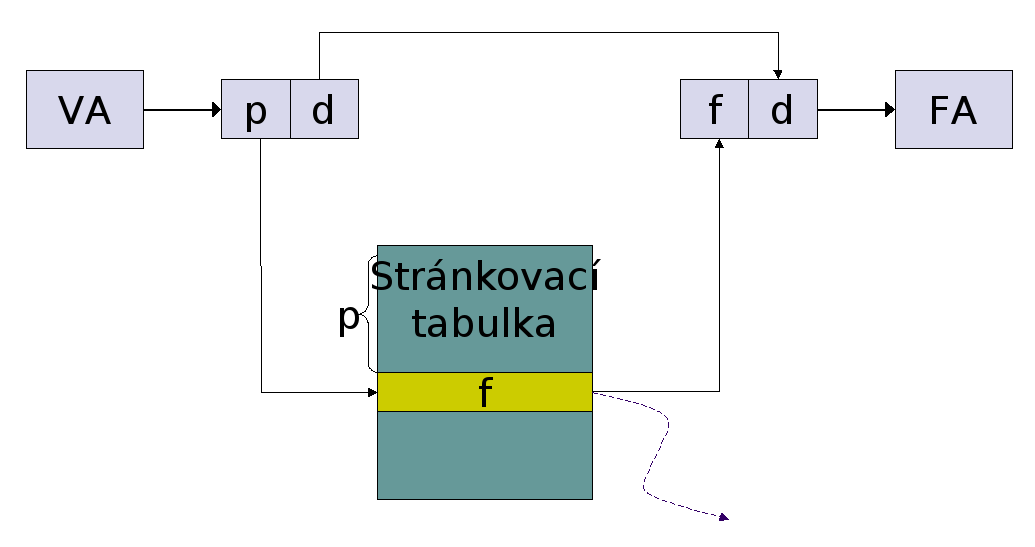
\includegraphics[width=10cm]{informatika/operacne_systemy_a_hw/obrazky/strankovani1.png}\end{center}
	\item umožnuje \emph{oddělené VAP} i \emph{sdílenou paměť} - mapování virtuální stránky 2 procesů na jednu fyzickou
	\item víceúrovňové stránkování (např. kvůli velikosti)
		\par \begin{center} 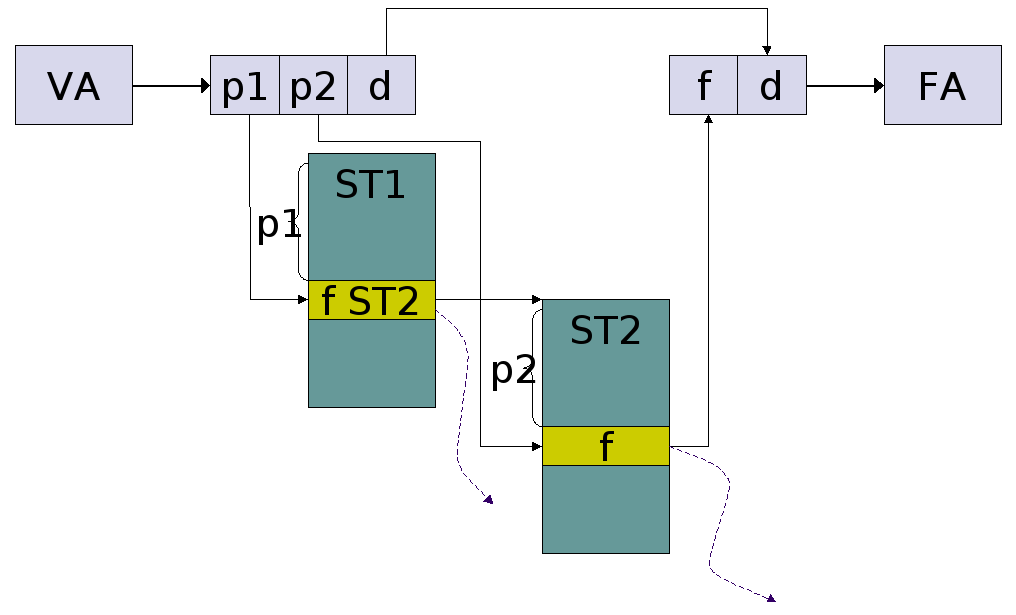
\includegraphics[width=10cm]{informatika/operacne_systemy_a_hw/obrazky/strankovani2.png} \end{center}
	\item TLB (Translation Lookaside Buffer) - asociativní paměť sloužící na rychlé vyhledání mapování virtuální stránky na fyzickou, využívá lokalitu chování programů
		\par \begin{center} 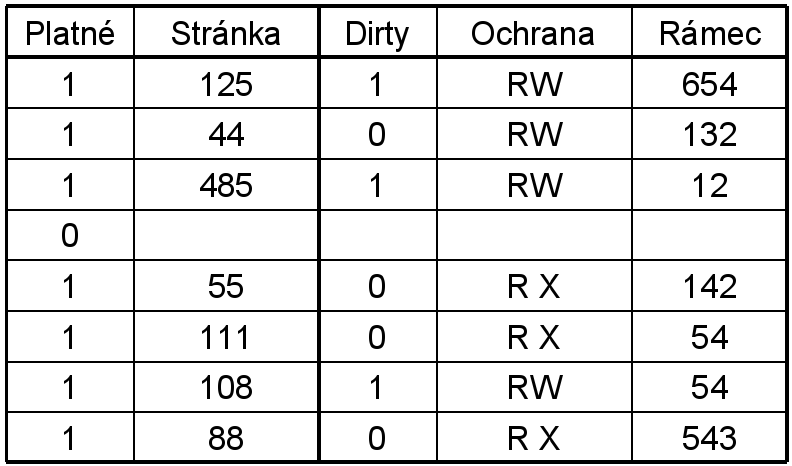
\includegraphics[width=6cm]{informatika/operacne_systemy_a_hw/obrazky/strankovani-tlb.png} \end{center} 
		\par ...nulaúrovňové stránkování - používá pouze TLB, řízeno také OS (oblíbené u 64-bitových CPU - UltraSPARC III)
	\item inverzní stránkování (např. když FAP je menší než VAP, 64-bitové CPU - IA-64)
		\par \begin{center} 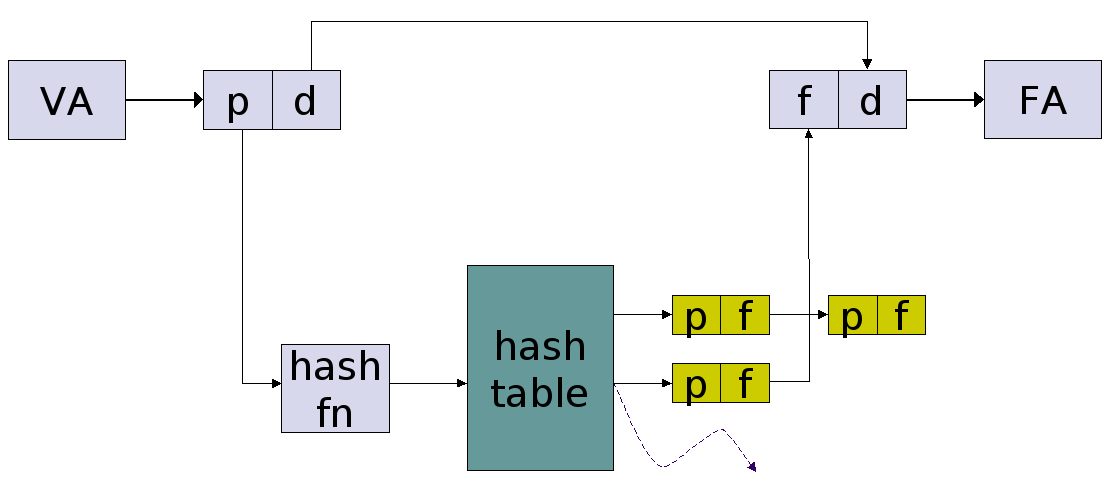
\includegraphics[width=10cm]{informatika/operacne_systemy_a_hw/obrazky/strankovani-inv.png} \end{center} 
\end{pitemize}

Akce vykonávané při výpadku stránky:
\begin{pitemize}
	\item výjimka procesoru
	\item uložit stav CPU (kontext)
	\item zjistit VA
	\item kontrola platnosti adresy a práv
	\item nalezení volného rámce
	\item zrušit mapování na nalezený rámec
	\item pokud je vyhazovaný rámec vyhazován, spustit ukládání na disk
	\item načíst z disku požadovanou stránku do rámce
	\item zavést mapování
	\item obnovit kontext
\end{pitemize}


Při implementaci stránkování je nutno brat v úvahu: 
\begin{pitemize}
    \item \emph{znovuspuštění instrukce} --- je potřeba aby procesor po výpadku zkusil přístup do paměti znova. dnes umí všechny CPU, např. 68xxx - problémy (přerušení v půlce instrukce) 
    \item \emph{sdílení stránek} --- jednomu rámci odp. víc stránek $\rightarrow$ pokud s ním něco dělám, týká se to všech stránek!  musím vše ost. odmapovat. musím si pamatovat mapování pro každý rámec - obrácené tabulky. 
    \item \emph{odstranění položky z TLB při rušení mapování} --- nestačí změnit tabulky, musí se vyhodit i z TLB (kde to může, ale nemusí být). problém - u multiprocesorů má každá CPU vlastní TLB, tabulky jsou sdílené $\rightarrow$ CPU při rušení mapování musí poslat interrupt s rozkazem ke smazání všem (i sobě), počkat na potvrzení akce od všech.
\end{pitemize}

\subsubsection*{Algoritmy pro výměnu stránek}
\begin{pitemize}
	\item \textbf{Optimální stránka} (v okamžiku výpadku stránky vybírám stránku, na níž se přistoupí za největší počet instrukcí) - nelze implementovat
	\item \textbf{NRU} (Not Recently Used) - každá stránka má příznaky Accessed a Dirty (typicky implementovatelné v HW, možno simulovat SW); jednou za čas se smažou všechna A; při výpadku rozdělím stránky podle A,D a vyberu stránku z nejnižší neprázdné třídy:
		\par \begin{center}
		\begin{tabular}{|c|c|c|}
			\hline 
			  & A & D \\
			\hline
			0 & 0 & 0 \\
			\hline
			1 & 0 & 1 \\
			\hline
			2 & 1 & 0 \\
			\hline
			3 & 1 & 1 \\
			\hline
		\end{tabular}
		\end{center}
	\item \textbf{FIFO} (vykazuje anomálie - Belady (zvětšení počtu výpadků stránky, když zvýšíme počet stránek v paměti)), druhá šance (úprava FIFO; pokud A=1, zařadím na konec FIFO... nevykazuje anomálie)
	\item \textbf{Hodiny} - modifikace druhé šance: kruhový zoznam stránek + iterátor na ukazující na nejstarší stránku v zoznamu. Při výpadku (a neexistenci volého rámce) se zjistí, jestli má *iterator nastavený příznak Accessed. Jestli ne, tato stránka bude nahrazena - v opačném případě se Accessed příznak zruší a iterator++. Toto se opakuje, dokud nedojde k výměně\dots
	\item \textbf{LRU} (Least Recently Used) - často používané stránky v posledním krátkém časovém úšeku budou znovu použity, čítač použití stránek, možné implementovat v HW
	\item \textbf{NFU} (Not Frequently Used) - SW simulace LRU, SW čítač ke každé stránce; jednou za čas projdu všechna A a přičtu je k odpovídajícím čítačům; vybírám stránku s nejnižším čítačem; nezapomíná - je možná modifikace se stárnutím čítače
\end{pitemize}

\subsubsection*{Segmentace}
dnes pouze Intel IA-32, dvojrozměrný VAP
\begin{pitemize}
	\item rozdělení programu na segmenty (napr. podle částí s různými vlastnostmi - kód, data, zásobníky\dots), různé délky segmentů, ktoré můžou měnit svoji délku za běhu
	\item VAP dvourozměrný (segment, offset), FAP jednorozměrný (vyzerá jako při spojitém pridělování paměti)
	\item segmentová převodní tabulka (VA se skládá ze dvou častí S:D, v tabulce se najde adresa segmentu S\dots k této adrese se poté přičte D, co je umístnění adresy v FA), příznak existence mapování
	\item při výpadku je nutné měnit celý segment (ty mohou být velké), je možné segmenty sesypat - ale nelze mít segment větší než FAP
\end{pitemize}

Segmentaci je možné kombinovat se stránkováním (odstraňuje nevýhody segmentace, neprovádí se výpadky segmentů):
\par \begin{center}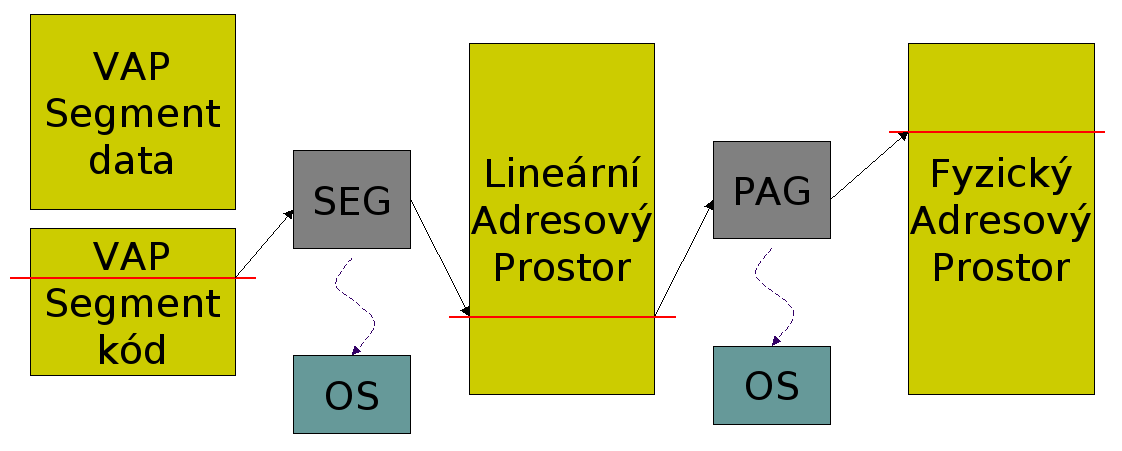
\includegraphics[width=12cm]{informatika/operacne_systemy_a_hw/obrazky/segmentace-a-strankovani.png}\end{center}
